\chapter{Statistical Modeling of Solutions}\label{chapter:bayesian}

\section{Introduction}

The OverCode work began with the vision that a teacher would someday be able to look at a display summarizing hundreds or thousands of student solutions to the same problem and immediately see---and comment on---good and bad design decisions that students made. There will be some design decisions within each solution that are rare and some that are common, some that exemplify good programming practices and others that do not. These decisions might create inefficient solutions, reveal a student's fundamental misunderstanding, or use a feature of the language in a creative way.

Hundreds or thousands of solutions to the same introductory python programming prompt can share a lot of structure and behavior. Empirically, the number of different design decisions made by students can be relatively small, or at least distributed in such a way that the majority of students' decisions fall into a small number of categories, with the remaining students making much more unique design choices. 

However, the number of distinct student solutions grows exponentially with the number of locations in the program where students do not all make the same design decision. The OverCode canonicalization and stacking pipeline reduces the number of distinct solutions by collapsing dimensions that exist only because of differences in variable names or behaviorally equivalent statement orders. The pipeline helps reduce the number of student solutions a teacher needs to consider, but it does not fulfill the original vision: turning thousands of solutions into a small set of solution exemplars or facets of solutions that exemplify the underlying student design decisions.

Given the relatively small set of underlying design decisions, the common structures shared by many student solutions, the availability of feature vectors already computed by the OverCode pipeline, and earlier promising experimentation with Bayesian non-parametric methods as part of a collaboration with \citet{beenthesis}, Bayesian non-parametric methods may be key to fulfilling the original vision for OverCode.

\section{Empirical Qualities of Solution Clusters}

Clustering python solutions has a strong subjective component. In early pilot studies, python programming teachers given the same set of solutions partitioned the space of solutions in a variety of ways, producing different numbers and/or compositions of clusters. Since teachers found multiple reasonable clusterings, the pilot results can be explained by one or both of the following reasons: (1) Teachers have different internal clustering metrics. (2) Given a clustering metric, solutions can still belong to multiple clusters.

It is also reasonable to assume that, given additional solutions to the same programming problem, some solutions would fall into existing clusters and some would represent wholly new solution successes or failures. It is reasonable to assume there is not some true total number of clusters that one reaches if one sees enough data.

\section{Relevant Bayesian Models}

There are a variety of Bayesian methods that can handle one or more of the difficulties of clustering python solutions. The following methods are potentially good fits: 
\begin{itemize}
\item Latent Dirichlet Allocation (LDA) models solutions as "documents" with sets of "words," where each word belongs to one topic and each document can contain words from multiple topics.
\item Dirichlet Process Mixture Models (DPMMs) do not require the number of clusters to be set beforehand; the number of clusters solutions are assigned to can grow as the number of solutions grow. However, every data point belongs to one cluster.
\item Hierarchical Dirichlet Process Models (HDPs), like DPMMs, do not require a pre-set number of clusters. Unlike DPMMs, solutions do not belong to a single cluster. Like LDA, solutions contain features, and each feature belongs to a cluster. Solutions can contain features from multiple clusters. This method emulates LDA with no pre-set number of clusters. 
\item Models and inference algorithms built on Indian Buffet Processes (IBPs) by \citet{doshi2009indian} are like HDPs, but allow individual features can belong to multiple clusters.
\item Bayesian Case Models (BCM) \citet{beenthesis} learn a pre-set number of subspace clusters, where each cluster is represented by an example and a small set of features that play an "important role" in identifying that cluster \citet{beenNIPS}. This representation of the clusters has been designed to increase human interpretability of the results. This model has has an interactive version, iBCM \cite{beenthesis}, where humans can directly modify the cluster example and important features that characterize a cluster.
\item Mind the Gap model (MGM) by \citet{kim2015mind} clusters data while also learning a "global set of distinguishable dimensions to assist with further data exploration and hypothesis generation."
\end{itemize}

\section{Model Choice}

Since (1) we do not know how many clusters will exist in the data ahead of time and (2) new solutions may introduce new clusters (there is no finite limit on the number of clusters as more solutions are received), models built on Dirichlet Processes are a good fit. 

Since solutions may contain multiple design decisions, it is preferable to be able to assign each of those design decisions separately, rather than assigning the entire solution to a cluster. HDPs are a good fit. If different design decisions share common features, IBPs may be an even better fit.

Since the output of LDA and its infinite cousin, the HDP, can be difficult to interpret, BCM or MGM's optimizations for interpretability may make them more appropriate choices.

Since teachers develop their own internal rubric for which differences matter and which do not, models which can incorporate and adjust based on feedback from the user, like iBCM, may be good model choices.

Each of these models have favorable properties, and some properties can be super-imposed, while others are mutually exclusive. There is also previously ignored factors like the difficulty of implementing an inference algorithm for the model and the scalability and time requirements of running the chosen inference algorithm on the chosen representation of the solutions.

\section{Feature Choice}

Once a collection of solutions to the same problem have been processed by the OverCode pipeline, there are a variety of features that can be used to describe each solution, including but not limited to canonicalized variables and lines. 

I am chosing to initially focus on the feature space defined by which canonicalized variables appear in each solution. This feature space has the lowest number of dimensions of the three solution representations just mentioned; there are only several hundred canonicalized variables across several thousand solutions to a particular problem of computing a derivative. I am mindful of this ratio, because as the number of features relative to solutions increases, the curse of dimensionality may wreck havoc. Figure \ref{fig:solutions_variables_pca} is a visualization of these solutions, and there are already some visible clusters. A similar variable-based feature space has been successfully used before by Taherkhani et al. \cite{taherkhani13}, though it was eventually augmented by their equivalent of canonicalized lines.

\begin{figure}
     \centering
  	 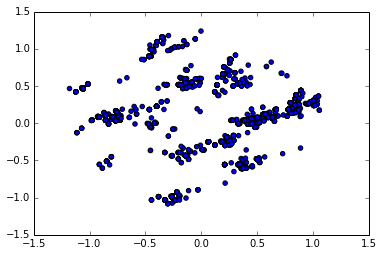
\includegraphics[width=\textwidth]{Body/figures/pca_of_solution_variables.png}
     \caption[PCA on Solutions Represented by Abstract Variables]{This represents the two most significant dimensions of PCA applied to several thousand solutions to the same problem that are represented by the variables they contain.}
     \label{fig:solutions_variables_pca}
\end{figure}

\begin{comment}
\section{Plan for Applying Models to Solution Collections}

\begin{enumerate}

\item I implemented a DP-stick-breaking/GEM distribution generator.
\item I studied and understood the stick-breaking construction of the Hierarchical Dirichlet Process found in Section 4.1 of the article Hierarchical Dirichlet Processes by \citet{hdp05}.
\item By April 22nd, I will implement and test, in python, either (1) the Gibbs sampler for CRPs implemented in R and demonstrated in the third MLSS '15 lecture on Bayesian nonparametric statistics or (2) the second algorithm in \citet{neal2000markov}, which performs Gibbs sampling on DPMMs with conjugate priors.
\item By May 4th, I will then generalize the same implementation from the previous step to add a level of hierarchy, in order to perform clustering by Hierarchical Dirichlet Processes. 
\item By May 10th, I will write up the algorithm and its performance on python solutions.
\end{enumerate}

I do have stretch goals, as incentives to finish more quickly, specifically: (1) adding the subspace-learning feature of BCMs to my implementation and (2) predicting rubric labels teaching assistants will apply, based on the labels actually applied by teaching assistants during grading with OverCode.
\end{comment}

%\section{Predicting Rubric Labels}


